\ifx\wholebook\relax \else
% ------------------------ 

\documentclass{article}
%------------------- Other types of document example ------------------------
%
%\documentclass[twocolumn]{IEEEtran-new}
%\documentclass[12pt,twoside,draft]{IEEEtran}
%\documentstyle[9pt,twocolumn,technote,twoside]{IEEEtran}
%
%-----------------------------------------------------------------------------
%%
% loading packages
%
\newif\ifpdf
\ifx\pdfoutput\undefined % We're not running pdftex
  \pdffalse
\else
  \pdftrue
\fi
%
%
\ifpdf
  \RequirePackage[pdftex,%
            CJKbookmarks,%
       bookmarksnumbered,%
              colorlinks,%
          linkcolor=blue,%
              hyperindex,%
        plainpages=false,%
       pdfstartview=FitH]{hyperref}
\else
  \RequirePackage[dvipdfm,%
             CJKbookmarks,%
        bookmarksnumbered,%
               colorlinks,%
           linkcolor=blue,%
               hyperindex,%
         plainpages=false,%
        pdfstartview=FitH]{hyperref}
  \AtBeginDvi{\special{pdf:tounicode GBK-EUC-UCS2}} % GBK -> Unicode
\fi
\usepackage{hyperref}

% other packages
%-----------------------------------------------------------------------------
\usepackage{graphicx, color}
\usepackage{CJK}
%
% for programming 
%
\usepackage{verbatim}
\usepackage{listings}


\lstdefinelanguage{Smalltalk}{
  morekeywords={self,super,true,false,nil,thisContext}, % This is overkill
  morestring=[d]',
  morecomment=[s]{"}{"},
  alsoletter={\#:},
  escapechar={!},
  literate=
    {BANG}{!}1
    {UNDERSCORE}{\_}1
    {\\st}{Smalltalk}9 % convenience -- in case \st occurs in code
    % {'}{{\textquotesingle}}1 % replaced by upquote=true in \lstset
    {_}{{$\leftarrow$}}1
    {>>>}{{\sep}}1
    {^}{{$\uparrow$}}1
    {~}{{$\sim$}}1
    {-}{{\sf -\hspace{-0.13em}-}}1  % the goal is to make - the same width as +
    %{+}{\raisebox{0.08ex}{+}}1		% and to raise + off the baseline to match -
    {-->}{{\quad$\longrightarrow$\quad}}3
	, % Don't forget the comma at the end!
  tabsize=2
}[keywords,comments,strings]

\lstloadlanguages{C++, Lisp, Smalltalk}

% ======================================================================

\def\BibTeX{{\rm B\kern-.05em{\sc i\kern-.025em b}\kern-.08em
    T\kern-.1667em\lower.7ex\hbox{E}\kern-.125emX}}

\newtheorem{theorem}{Theorem}

%
% mathematics
%
\newcommand{\be}{\begin{equation}}
\newcommand{\ee}{\end{equation}}
\newcommand{\bmat}[1]{\left( \begin{array}{#1} }
\newcommand{\emat}{\end{array} \right) }
\newcommand{\VEC}[1]{\mbox{\boldmath $#1$}}

% numbered equation array
\newcommand{\bea}{\begin{eqnarray}}
\newcommand{\eea}{\end{eqnarray}}

% equation array not numbered
\newcommand{\bean}{\begin{eqnarray*}}
\newcommand{\eean}{\end{eqnarray*}}

\RequirePackage{CJK,CJKnumb,CJKulem,CJKpunct}
% we use CJK as default environment
\AtBeginDocument{\begin{CJK*}{GBK}{song}\CJKtilde\CJKindent\CJKcaption{GB}}
\AtEndDocument{\clearpage\end{CJK*}}

%
% loading packages
%
\newif\ifpdf
\ifx\pdfoutput\undefined % We're not running pdftex
  \pdffalse
\else
  \pdftrue
\fi
%
%
\ifpdf
  \RequirePackage[pdftex,%
       bookmarksnumbered,%
              colorlinks,%
          linkcolor=blue,%
              hyperindex,%
        plainpages=false,%
       pdfstartview=FitH]{hyperref}
\else
  \RequirePackage[dvipdfm,%
        bookmarksnumbered,%
               colorlinks,%
           linkcolor=blue,%
               hyperindex,%
         plainpages=false,%
        pdfstartview=FitH]{hyperref}
\fi
\usepackage{hyperref}

% other packages
%-----------------------------------------------------------------------------
\usepackage{graphicx, color}
%
% for programming 
%
\usepackage{verbatim}
\usepackage{listings}
\usepackage{algorithmic} %for pseudocode
\usepackage{algorithm}


\lstdefinelanguage{Smalltalk}{
  morekeywords={self,super,true,false,nil,thisContext}, % This is overkill
  morestring=[d]',
  morecomment=[s]{"}{"},
  alsoletter={\#:},
  escapechar={!},
  literate=
    {BANG}{!}1
    {UNDERSCORE}{\_}1
    {\\st}{Smalltalk}9 % convenience -- in case \st occurs in code
    % {'}{{\textquotesingle}}1 % replaced by upquote=true in \lstset
    {_}{{$\leftarrow$}}1
    {>>>}{{\sep}}1
    {^}{{$\uparrow$}}1
    {~}{{$\sim$}}1
    {-}{{\sf -\hspace{-0.13em}-}}1  % the goal is to make - the same width as +
    %{+}{\raisebox{0.08ex}{+}}1		% and to raise + off the baseline to match -
    {-->}{{\quad$\longrightarrow$\quad}}3
	, % Don't forget the comma at the end!
  tabsize=2
}[keywords,comments,strings]

\lstloadlanguages{C++, Lisp, Haskell, Python, Smalltalk}

% ======================================================================

\def\BibTeX{{\rm B\kern-.05em{\sc i\kern-.025em b}\kern-.08em
    T\kern-.1667em\lower.7ex\hbox{E}\kern-.125emX}}

\newtheorem{theorem}{Theorem}

%
% mathematics
%
\newcommand{\be}{\begin{equation}}
\newcommand{\ee}{\end{equation}}
\newcommand{\bmat}[1]{\left( \begin{array}{#1} }
\newcommand{\emat}{\end{array} \right) }
\newcommand{\VEC}[1]{\mbox{\boldmath $#1$}}

% numbered equation array
\newcommand{\bea}{\begin{eqnarray}}
\newcommand{\eea}{\end{eqnarray}}

% equation array not numbered
\newcommand{\bean}{\begin{eqnarray*}}
\newcommand{\eean}{\end{eqnarray*}}




\setcounter{page}{1}

\begin{document}

\fi
%--------------------------

% ================================================================
%                 COVER PAGE
% ================================================================

\title{Red-black tree, not so complex as it was thought}

\author{Liu~Xinyu
\thanks{{\bfseries Liu Xinyu } \newline
  Email: liuxinyu95@gmail.com \newline}
  }

\markboth{Red black tree}{AlgoXY}

\maketitle

\ifx\wholebook\relax
\chapter{Red-black tree, not so complex as it was thought}
\fi

% ================================================================
%                 Introduction
% ================================================================
\section{Introduction}
\label{introduction} \index{red-black tree}

\subsection{Exploit the binary search tree}
We have shown the power of binary search tree by using it to count
the occurrence of every word in Bible. The idea is to use binary
search tree as a dictionary for counting.

One may come to the idea that to feed a yellow page book
\footnote{A name-phone number contact list book} to a binary
search tree, and use it to look up the phone number for a contact.

By modifying a bit of the program for word occurrence counting
yields the following code.

\begin{lstlisting}
int main(int, char** ){
  ifstream f("yp.txt");
  map<string, string> dict;
  string name, phone;
  while(f>>name && f>>phone)
    dict[name]=phone;
  for(;;){
    cout<<"\nname: ";
    cin>>name;
    if(dict.find(name)==dict.end())
      cout<<"not found";
    else
      cout<<"phone: "<<dict[name];
  }
}
\end{lstlisting}

This program works well. However, if you replace the STL map 
with the binary search tree as mentioned previously, the 
performance will be bad, especially when you search some names such
as Zara, Zed, Zulu.

This is because the content of yellow page is typically listed
in lexicographic order. Which means the name list is in increase
order. If we try to insert a sequence of number 1, 2, 3, ..., n 
to a binary search tree. We will get a tree like in Figure \ref{fig:unbalanced-tree}.

\begin{figure}[htbp]
       \begin{center}
	\includegraphics[scale=0.5]{img/unbalanced.ps}
        \caption{unbalanced tree} \label{fig:unbalanced-tree}
       \end{center}
\end{figure}

This is a extreme unbalanced binary search tree. The looking up performs
$O(h)$ for a tree with height $h$. In balanced case, we benefit from 
binary search tree by $O(\lg N)$ search time. But in this extreme case, 
the search time downgraded to $O(N)$. It's no better than a normal link-list.

\subsection*{Exercise}

\begin{itemize}
\item For a very big yellow page list, one may want to speed up the
dictionay building process by two concurrent tasks (threads or processes).
One task reads the name-phone pair from the head of the list, while the
other one reads from the tail. The building terminates when these
two tasks meet at the middle of the list. What will be the binary
search tree looks like after building? What if you splite the the
list more than two and use more tasks?

\item Can you find any more cases to exploit a binary search tree?
Please consider the unbalanced trees shown in figure 
\ref{fig:unbalanced-trees}.
\end{itemize}

\begin{figure}[htbp]
       \begin{center}
       \includegraphics[scale=0.5]{img/unbalanced-2.ps} \includegraphics[scale=0.5]{img/unbalanced-zigzag.ps} \\
       \includegraphics[scale=0.5]{img/unbalanced-3.ps} 
       \caption{Some unbalanced trees} \label{fig:unbalanced-trees}
       \end{center}
\end{figure}

\subsection{How to ensure the balance of the tree}
In order to avoid such case, we can shuffle the input sequence by 
randomized algorithm, such as described in Section 12.4 in \cite{CLRS}.
However, this method doesn't always work, for example the input is fed 
from user interactively, and the tree need to be built/updated after each input.

There are many solutions people have ever found to make binary search tree balanced.
Many of them rely on the rotation operations to binary search tree. 
Rotation operations change the tree structure while maintain the ordering
of the elements. Thus it either improve or keep the balance property of the binary
search tree.

In this chapter, we'll first introduce about red-black tree, which is one of the 
most popular and widely used self-adjusting blanced 
binary search tree. In next chapter, we'll introduce about AVL tree, which is 
another intuitive solution; In later chapter about binary heaps, we'll show another 
interesting tree called splay tree, which can gradually adjust the the tree to make it
more and more balanced.

\subsection{Tree rotation}
\index{tree rotation}

\begin{figure}[htbp]
       \begin{center}
       \includegraphics[scale=0.4]{img/rotate-r.ps} \includegraphics[scale=0.4]{img/rotate-l.ps} 
       \caption{Tree rotation, `rotate-left' transforms the tree from left side to right side, and `rotate-right' does the inverse transformation.} \label{fig:tree-rotation}
       \end{center}
\end{figure}

Tree rotation is a kind of special operation that can transform the tree structure
without changing the in-order traverse result. It based on the fact that
for a specified ordering, there are multiple binary search trees correspond to it.
Figure \ref{fig:tree-rotation} shows the tree rotation. For a binary search tree
on the left side, left rotate transforms it to the tree on the right, and right
rotate does the inverse transformation.

Although tree rotation can be realized in procedural way, there exists quite 
simple function description if using pattern matching.

\be
rotateL(T) = \left \{
  \begin{array}
  {r@{\quad:\quad}l}
  node(node(a, X, b), Y, c) & pattern(T) = node(a, X, node(b, Y, c)) \\
  T & otherwise
  \end{array}
\right .
\ee

\be
rotateR(T) = \left \{
  \begin{array}
  {r@{\quad:\quad}l}
  node(a, X, node(b, Y, c)) & pattern(T) = node(node(a, X, b), Y, c)) \\
  T & otherwise
  \end{array}
\right .
\ee

However, the pseudo code dealing imperatively has to set all fields accordingly.

\begin{algorithmic}
\Function{Left-Rotate}{$T, x$}
  \State $p \gets$ \Call{Parent}{$x$}
  \State $y \gets$ \Call{Right}{$x$} \Comment{Assume $y \ne NIL$}
  \State $a \gets$ \Call{Left}{$x$}
  \State $b \gets$ \Call{Left}{$y$}
  \State $c \gets$ \Call{Right}{$y$}
  \State \Call{Replace}{$x, y$}
  \State \Call{Set-Children}{$x, a, b$}
  \State \Call{Set-Children}{$y, x, c$}
  \If{$p = NIL$}
    \State $T \gets y$
  \EndIf
  \State \Return $T$
\EndFunction

\Statex

\Function{Right-Rotate}{$T, y$}
  \State $p \gets$ \Call{Parent}{$y$}
  \State $x \gets$ \Call{Left}{$y$} \Comment{Assume $x \ne NIL$}
  \State $a \gets$ \Call{Left}{$x$}
  \State $b \gets$ \Call{Right}{$x$}
  \State $c \gets$ \Call{Right}{$y$}
  \State \Call{Replace}{$y, x$}
  \State \Call{Set-Children}{$y, b, c$}
  \State \Call{Set-Children}{$x, a, y$}
  \If{$p = NIL$}
    \State $T \gets x$
  \EndIf
  \State \Return $T$
\EndFunction

\Statex

\Function{Set-Left}{$x, y$}
  \State \Call{Left}{$x$} $\gets y$
  \If{$y \ne NIL$}
    \Call{Parent}{$y$} $\gets x$
  \EndIf
\EndFunction

\Statex

\Function{Set-Right}{$x, y$}
  \State \Call{Right}{$x$} $\gets y$
  \If{$y \ne NIL$}
    \Call{Parent}{$y$} $\gets x$
  \EndIf
\EndFunction

\Statex

\Function{Set-Children}{$x, L, R$}
  \State \Call{Set-Left}{$x, L$}
  \State \Call{Set-Right}{$x, R$}
\EndFunction

\Statex

\Function{Replace}{$x, y$}
  \If{\Call{Parent}{$x$} $= NIL$}
    \If{$y \ne NIL$}
      \Call{Parent}{$y$} $\gets NIL$
    \EndIf
  \ElsIf{\textproc{Left}(\Call{Parent}{$x$}) $= x$}
    \textproc{Set-Left}(\Call{Parent}{$x$}, $y$)
  \Else
    \textproc{Set-Right}(\Call{Parent}{$x$}, $y$)
  \EndIf
  \State \Call{Parent}{$x$} $\gets NIL$
\EndFunction
\end{algorithmic}

Compare these pseudo codes with the pattern matching functions, 
the former focus on the structure states changing, while the 
latter focus on the rotation process. As the title of this 
chatper indicated, red-black tree needn't be so complex as it 
was thought. Most traditional algorithm text books use the 
classic procedural way to teach red-black tree, there are 
serveral cases need to deal and all need carefulness to 
manipulate the node fields. However, by chaning
the mind to functional settings, things get intuitive and
simple. Altough there is some performance overhead.

Most of the content in this chapter is based on Chris Okasaki's
work in \cite{okasaki}.

% ================================================================
% Definition
% ================================================================
\section{Definition of red-black tree}
\index{red-black tree}

Red-black tree is a type of self-balancing binary search tree\cite{wiki}. 
\footnote{Red-black tree is one of the equivalent form of 2-3-4 tree (see chapter
B-tree about 2-3-4 tree). That is to say, for any 2-3-4 tree, there is at least 
one red-black tree has the same data order.} By using color changing and rotation, 
red-black tree provides a very simple and straightforward way to keep 
the tree balanced.

For a binary search tree, we can augment the nodes with a color field, a node
can be colored either red or black. We call a binary search tree red-black tree 
if it satisfies the following 5 properties\cite{CLRS}.

\begin{enumerate}
\item Every node is either red or black.
\item The root is black.
\item Every leaf (NIL) is black.
\item If a node is red, then both its children are black.
\item For each node, all paths from the node to descendant leaves contain the same number of black nodes.
\end{enumerate}

Why this 5 properties can ensure the red-black tree is well balanced? 
Because they have a key characteristic, the longest path from root to 
a leaf can't be as 2 times longer than the shortest path.

Please note the 4th property, which means there won't be two adjacent 
red nodes. so the shortest path only contains black nodes, any paths 
longer than the shortest one has interval red nodes. According to 
property 5, all paths have the same number of black nodes, 
this finally ensure there won't be any path is 2 times longer than 
others\cite{wiki}. Figure \ref{fig:rbt-example} shows an example
red-black tree.

\begin{figure}[htbp]
       \begin{center}
	\includegraphics[scale=0.5]{img/rbt-example.ps}
        \caption{An example red-black tree} \label{fig:rbt-example}
       \end{center}
\end{figure}

All read only operations such as search, min/max are as same as in 
binary search tree. While only the insertion and deletion are special.

As we have shown in word occurrence example, many implementation of 
set or map container are based on red-black tree. One example is the 
C++ Standard library (STL)\cite{sgi-stl}. 

As mentioned previously, the only change in data layout is that
there is color information augumented to binary search tree.
This can be represented as a data field in imperative languages
such as Python like below.

TODO: change to C++ code

\lstset{language=Python}
\begin{lstlisting}
class Node:
    def __init__(self, key, color = RED):
        self.key = key;
        self.color = color;
        self.left = self.right = self.parent = None
\end{lstlisting}

And in functional settings, we can add the color information
in constructors, below is the Haskell example of red-black tree
definition.

\lstset{language=Haskell}
\begin{lstlisting}
data Color = R | B deriving (Show, Eq) 
data RBTree a = Empty
              | Node Color (RBTree a) a (RBTree a)
\end{lstlisting}

TODO: ...

% ================================================================
%                 Insertion
% ================================================================
\section{Insertion}

Insertion can violate the red black tree properties, so we need transform
the tree after insertion.

We can use the same insert function as defined in binary search tree, and 
then do some fix the resume the red black properties. One good practice is 
to always insert red node. as far as the new inserted node isn't the root.
We can keep all properties except number 4. It may bring two adjacent red
nodes.

Functional and imperative implementation have different fixing ways. One
is uniformed but has some overhead, the other is a bit complex but has 
higher performance.

\subsubsection*{Haskell red black insertion, functional}
As described by Chris Okasaki, there are total 4 cases which violate property 4.
All of them has 2 adjacent red nodes. However, they have a uniformed form
after fixing\cite{okasaki}. 

\begin{figure}[htbp]
       \begin{center}
	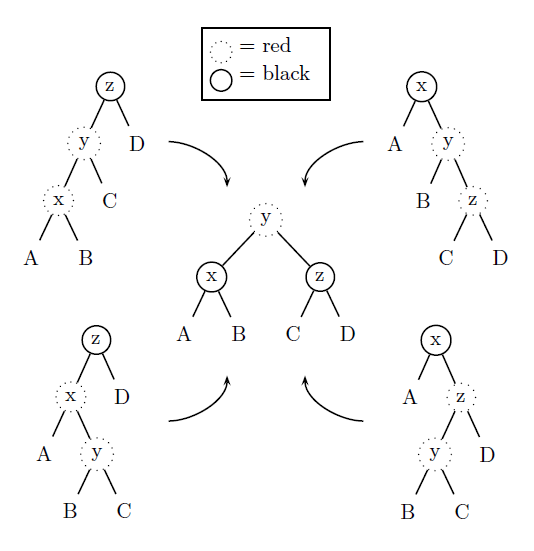
\includegraphics[scale=0.5]{img/insert-fix.eps}
        \caption{4 cases for balancing a red black tree after insertion} \label{fig:insert-fix}
       \end{center}
\end{figure}

Note that this transformation will move the redness one level up. So this is a bottom-up recursive fixing, the last step will make the root node red. According
to property 2, root is always black. So we need final fixing to revert the root
color to black. All these can be implemented as the following Haskell code.

\lstset{language=Haskell}
\begin{lstlisting}
insert::(Ord a)=>RBTree a -> a -> RBTree a
insert t x = makeBlack(ins t x) where  --[1]
    ins Empty x = Node R Empty x Empty --[2]
    ins (Node color l k r) x 
        | x < k     = balance color (ins l x) k r
        | otherwise = balance color l k (ins r x) --[3]
    makeBlack(Node _ l k r) = Node B l k r

balance::Color -> RBTree a -> a -> RBTree a -> RBTree a
balance B (Node R (Node R a x b) y c) z d = 
                Node R (Node B a x b) y (Node B c z d)
balance B (Node R a x (Node R b y c)) z d = 
                Node R (Node B a x b) y (Node B c z d)
balance B a x (Node R b y (Node R c z d)) = 
                Node R (Node B a x b) y (Node B c z d)
balance B a x (Node R (Node R b y c) z d) = 
                Node R (Node B a x b) y (Node B c z d)
balance color l k r = Node color l k r
\end{lstlisting}

Here are some explanation. For [1], the program always set the root
color as black, this is because of property 2; For [2], we always insert
a red leaf to satisfy all properties except number 4; For [3], I assume, 
there shouldn't be different nodes with equal key value. But it is not always
applicable. for example in chapter 14, ``Augmenting Data Structures'' in CLRS\cite{CLRS}, it enables such case. The use of otherwise allows user to do this.

In order to test this program, we can write something like below.

\begin{lstlisting}
-- helper function to build a red black tree from a list

listToRBTree::(Ord a)=>[a] -> RBTree a
listToRBTree lst = foldl insert Empty lst

-- Helper function for pretty printing
instance Show a => Show (RBTree a) where
    show Empty = "."
    show (Node c l k r) = "(" ++ show l ++ " " ++ 
                          show k ++ ":" ++ show c ++ " " ++ 
                          show r ++ ")"

main = do
  putStrLn (show (listToRBTree [11, 2, 14, 1, 7, 15, 5, 8, 4]))
  putStrLn (show (listToRBTree [1, 2, 3, 4, 5, 6, 7, 8]))
\end{lstlisting}

This program will output:
\begin{verbatim}
(((. 1:B .) 2:B ((. 4:R .) 5:B .)) 7:B (((. 8:R .) 11:B .) 14:B (. 15:B .)))
(((. 1:B .) 2:B (. 3:B .)) 4:B ((. 5:B .) 6:B (. 7:B (. 8:R .))))
\end{verbatim}

They are trees as shown below.

\begin{figure}[htbp]
       \begin{center}
	\includegraphics[scale=0.4]{img/insert-haskell.ps}
        \caption{Haskell insert results} 
       \end{center}
\end{figure}

\subsubsection*{Scheme/Lisp red black tree insertion, functional}

Scheme/Lisp version of insert is very similar, since there is no pattern matching
in Scheme, we use normal condition to do the similar things.

\lstset{language=Lisp}
\begin{lstlisting}
(define (rb-insert tree x)
  (define (make-black t)
    (make-rbtree "B" (left t) (key t) (right t)))
  (define (ins t x)
    (cond ((null? t) (make-rbtree "R" '() x '()))
	  ((< x (key t)) (balance (color t) 
                                  (ins (left t) x) (key t) (right t)))
	  (else (balance (color t) (left t) (key t) (ins (right t) x)))))
  (make-black (ins tree x)))
\end{lstlisting}

And the core function balance which can fix the red-red violation is as below.

\begin{lstlisting}
(define (balance c l k r)
  (if (equal? c "B")
      (cond ((and (red? l) (red? (left l)))
	     (make-rbtree "R" 
			  (make-rbtree "B" (left (left l)) 
                                           (key (left l)) 
                                           (right (left l)))
			  (key l)
			  (make-rbtree "B" (right l) k r)))
	    ((and (red? l) (red? (right l)))
	     (make-rbtree "R"
			  (make-rbtree "B" (left l) (key l) (left (right l)))
			  (key (right l))
			  (make-rbtree "B" (right (right l)) k r)))
	    ((and (red? r) (red? (right r)))
	     (make-rbtree "R" 
			  (make-rbtree "B" l k (left r))
			  (key r)
			  (make-rbtree "B" (left (right r)) 
                                           (key (right r)) 
                                           (right (right r)))))
	    ((and (red? r) (red? (left r)))
	     (make-rbtree "R"
			  (make-rbtree "B" l k (left (left r)))
			  (key (left r))
			  (make-rbtree "B" (right (left r)) 
                                           (key r) 
                                           (right r))))
	    (else (make-rbtree c l k r)))
      (make-rbtree c l k r)))
\end{lstlisting}

This program can be test with a similar test cases as below:

\begin{lstlisting}
(define (list->rbtree lst)
  (fold-left rb-insert '() lst))

(define t1 (list->rbtree '(11 2 14 1 7 15 5 8 4)))
(define t2 (list->rbtree '(1 2 3 4 5 6 7 8)))
\end{lstlisting}

If we evaluate t1 and t2, it will output the results like this.

\begin{verbatim}
t1
;Value 11: (((() 1 "B" ()) 2 "B" ((() 4 "R" ()) 5 "B" ())) 7 "B" (((() 8 "R" ()) 
11 "B" ()) 14 "B" (() 15 "B" ())))

t2
;Value 12: (((() 1 "B" ()) 2 "B" (() 3 "B" ())) 4 "B" ((() 5 "B" ()) 6 "B" (() 
7 "B" (() 8 "R" ()))))
\end{verbatim}


\subsubsection*{Python red black tree insertion, imperative}

The python version imperative implementation uses the method described in CLRS.

\lstset{language=Python}
\begin{lstlisting}
def rb_insert(t, key): #returns the new root
    root = t
    x = Node(key)
    parent = None
    while(t):
        parent = t
        if(key < t.key):
            t = t.left
        else:
            t = t.right
    if parent is None: #tree is empty
        root = x
    elif key < parent.key:
        parent.set_left(x)
    else:
        parent.set_right(x)
    return rb_insert_fix(root, x)
\end{lstlisting}

Compare the above source code and the one in binary search tree\cite{bst-lxy}. The only difference are we simplified the program by using set\_left()/set\_right() member functions, and there is a rb\_insert\_fix() function call to fix the red node violation.

There are 3 cases described in CLRS, and if we take the left-right symmetric into consideration. there are total 6 cases. Among them two cases can be merged together, because they are all have uncle node in red color, we can toggle the parent color and uncle color to black and set grand parent color to red. After this merge the 5 cases fixing version can be implemented as the following.

\begin{lstlisting}
# Fix the red->red violation
def rb_insert_fix(t, x):
    while(x.parent and x.parent.color==RED):
        if x.uncle().color == RED:
            #case 1: ((a:R x:R b) y:B c:R) ==> ((a:R x:B b) y:R c:B)
            set_color([x.parent, x.grandparent(), x.uncle()],
                      [BLACK, RED, BLACK])
            x = x.grandparent()
        else:
            if x.parent == x.grandparent().left:
                if x == x.parent.right:
                    #case 2: ((a x:R b:R) y:B c) ==> case 3
                    x = x.parent
                    t=left_rotate(t, x)
                # case 3: ((a:R x:R b) y:B c) ==> (a:R x:B (b y:R c))
                set_color([x.parent, x.grandparent()], [BLACK, RED])
                t=right_rotate(t, x.grandparent())
            else:
                if x == x.parent.left:
                    #case 2': (a x:B (b:R y:R c)) ==> case 3'
                    x = x.parent
                    t = right_rotate(t, x)
                # case 3': (a x:B (b y:R c:R)) ==> ((a x:R b) y:B c:R)
                set_color([x.parent, x.grandparent()], [BLACK, RED])
                t=left_rotate(t, x.grandparent())
    t.color = BLACK
    return t
\end{lstlisting}

To test the insertion function. We use some similar helper functions and test functions defined in binary search tree\cite{bst-lxy}.

\begin{lstlisting}
def rbtree_clone(t):
    n = None
    if t != None:
        n = Node(t.key, t.color)
        n.set_children(rbtree_clone(t.left), rbtree_clone(t.right))
    return n

def rbtree_to_str(t):
    if t is None:
        return "."
    else:
        color = {RED:"R", BLACK:"B"}
        return "("+rbtree_to_str(t.left)+ " " + str(t.key) +":"+
               color[t.color]+" " + rbtree_to_str(t.right)+")"

def list_to_tree(l):
    tree = None
    for x in l:
        tree = rb_insert(tree, x)
    return tree

class Test:
    def __init__(self):
        self.t2=Node(11, BLACK) # as figure 13.4 in CLRS
        self.t2.set_children(Node(2), Node(14, BLACK))
        self.t2.left.set_children(Node(1, BLACK), Node(7, BLACK))
        self.t2.right.set_right(Node(15))
        self.t2.left.right.set_children(Node(5), Node(8))
        print "t2, CLRS fig 13.4:\n", rbtree_to_str(self.t2)

    def run(self):
        self.test_insert()

    def test_insert(self):
        t = rbtree_clone(self.t2)
        t = rb_insert(t, 4)
        print "t2: after insert 4\n", rbtree_to_str(t)
        t = list_to_tree([5, 2, 7, 1, 4, 6, 9, 3, 8])
        print "list->tree, create t1 by insert\n", rbtree_to_str(t)
\end{lstlisting}

Here we use the example tree present in CLRS as in figure \ref{fig:rb-insert-clrs}.

\begin{figure}[htbp]
       \begin{center}
	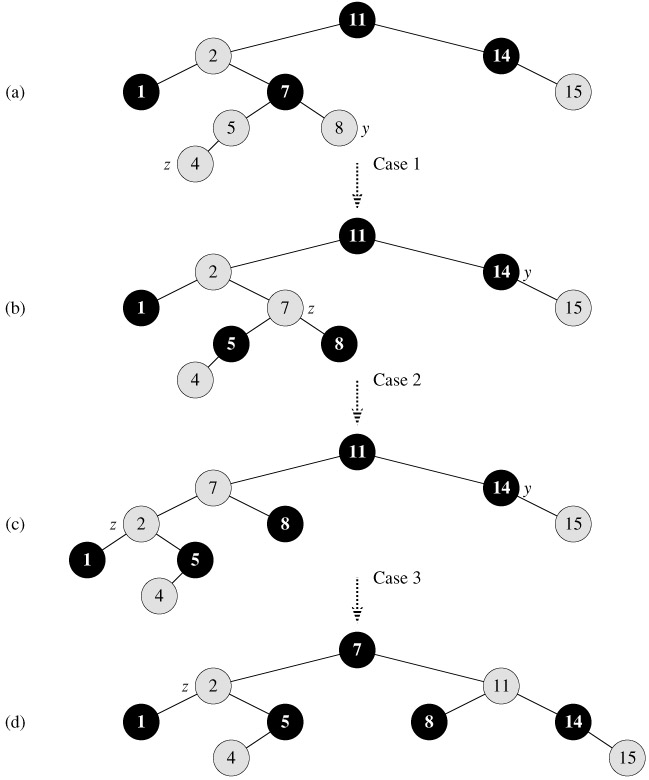
\includegraphics[scale=0.5]{img/rb-insert-clrs.eps}
        \caption{insertion and fixing} \label{fig:rb-insert-clrs}
       \end{center}
\end{figure}

The program will output 2 trees in console.

\begin{verbatim}
t2, CLRS fig 13.4:
(((. 1:B .) 2:R ((. 5:R .) 7:B (. 8:R .))) 11:B (. 14:B (. 15:R .)))
t2: after insert 4
(((. 1:B .) 2:R ((. 4:R .) 5:B .)) 7:B ((. 8:B .) 11:R (. 14:B (. 15:R .))))
list->tree, create t1 by insert
(((. 1:B .) 2:R ((. 3:R .) 4:B .)) 5:B ((. 6:B .) 7:R ((. 8:R .) 9:B .)))
\end{verbatim}

After insert element 4 into the first tree the result will be like in figure \ref{fig:rb-insert-clrs} (d), the second test case shows a tree which is created from a list as shown in figure \ref{fig:python-insert}.

\begin{figure}[htbp]
       \begin{center}
	\includegraphics[scale=0.5]{img/python-insert.ps}
        \caption{insert from a list} \label{fig:python-insert}
       \end{center}
\end{figure}

\subsubsection*{C++ red black tree insertion}

The C++ SGI STL implementation of red black tree also adopts the
concept of the sentinel as described in CLRS. Every time we initialize
an empty red black tree, it create such sentinel first.

\lstset{language=c++}
\begin{lstlisting}
void _M_empty_initialize() {
  _S_color(_M_header) = _S_rb_tree_red; // used to distinguish header from 
                                      // __root, in iterator.operator++
  _M_root() = 0;
  _M_leftmost() = _M_header;
  _M_rightmost() = _M_header;
}
\end{lstlisting}

Where the left sides are accessor operators, which returns the
reference of color, and other fields etc. There is a good explanation
in \cite{hj-stl}.

C++ SGI STL version of insertion provided two options,
insert\_unique() and insert\_equal(), we only present one of them in
this post.

\begin{lstlisting}
template <class _Key, class _Value, class _KeyOfValue, ...>
typename _Rb_tree<_Key,_Value,_KeyOfValue, ...>::iterator
_Rb_tree<_Key,_Value,_KeyOfValue, ...>
  ::insert_equal(const _Value& __v)
{
  _Link_type __y = _M_header;
  _Link_type __x = _M_root();
  while (__x != 0) {
    __y = __x;
    __x = _M_key_compare(_KeyOfValue()(__v), _S_key(__x)) ? 
            _S_left(__x) : _S_right(__x);
  }
  return _M_insert(__x, __y, __v);
}
\end{lstlisting}

In order to focus on the algorithm itself, I replace the allocator and
the compare template parameter with '...'. The insert will first use a 
while loop to locate where the new value should be inserted. then it
call \_M\_insert() function to do the real insertion. Where x is the
the insert position, y point to the parent of x.

Next, SGI STL will call the core insert function which is defined as
the following.

\begin{lstlisting}
template <class _Key, class _Value, class _KeyOfValue, ...>
typename _Rb_tree<_Key,_Value,_KeyOfValue, ...>::iterator
_Rb_tree<_Key,_Value,_KeyOfValue, ...>
  ::_M_insert(_Base_ptr __x_, _Base_ptr __y_, const _Value& __v)
{
  _Link_type __x = (_Link_type) __x_;
  _Link_type __y = (_Link_type) __y_;
  _Link_type __z;

  if (__y == _M_header || __x != 0 || 
      _M_key_compare(_KeyOfValue()(__v), _S_key(__y))) {
    __z = _M_create_node(__v);
    _S_left(__y) = __z;               // also makes _M_leftmost() = __z 
                                      //    when __y == _M_header
    if (__y == _M_header) {
      _M_root() = __z;
      _M_rightmost() = __z;
    }
    else if (__y == _M_leftmost())
      _M_leftmost() = __z;   // maintain _M_leftmost() pointing to min node
  }
  else {
    __z = _M_create_node(__v);
    _S_right(__y) = __z;
    if (__y == _M_rightmost())
      _M_rightmost() = __z;  // maintain _M_rightmost() pointing to max node
  }
  _S_parent(__z) = __y;
  _S_left(__z) = 0;
  _S_right(__z) = 0;
  _Rb_tree_rebalance(__z, _M_header->_M_parent);
  ++_M_node_count;
  return iterator(__z);
}
\end{lstlisting}

Most codes in this function deal with the leftmost and rightmost
members. They point to the minimum and maximum node in the tree. after
create the node with allocator, the program calls rebalance function
to fix the red-red violation.

\begin{lstlisting}
inline void 
_Rb_tree_rebalance(_Rb_tree_node_base* __x, _Rb_tree_node_base*& __root)
{
  __x->_M_color = _S_rb_tree_red;
  while (__x != __root && __x->_M_parent->_M_color == _S_rb_tree_red) {
    if (__x->_M_parent == __x->_M_parent->_M_parent->_M_left) {
      _Rb_tree_node_base* __y = __x->_M_parent->_M_parent->_M_right;
      if (__y && __y->_M_color == _S_rb_tree_red) {
        __x->_M_parent->_M_color = _S_rb_tree_black;
        __y->_M_color = _S_rb_tree_black;
        __x->_M_parent->_M_parent->_M_color = _S_rb_tree_red;
        __x = __x->_M_parent->_M_parent;
      }
      else {
        if (__x == __x->_M_parent->_M_right) {
          __x = __x->_M_parent;
          _Rb_tree_rotate_left(__x, __root);
        }
        __x->_M_parent->_M_color = _S_rb_tree_black;
        __x->_M_parent->_M_parent->_M_color = _S_rb_tree_red;
        _Rb_tree_rotate_right(__x->_M_parent->_M_parent, __root);
      }
    }
    else {
      _Rb_tree_node_base* __y = __x->_M_parent->_M_parent->_M_left;
      if (__y && __y->_M_color == _S_rb_tree_red) {
        __x->_M_parent->_M_color = _S_rb_tree_black;
        __y->_M_color = _S_rb_tree_black;
        __x->_M_parent->_M_parent->_M_color = _S_rb_tree_red;
        __x = __x->_M_parent->_M_parent;
      }
      else {
        if (__x == __x->_M_parent->_M_left) {
          __x = __x->_M_parent;
          _Rb_tree_rotate_right(__x, __root);
        }
        __x->_M_parent->_M_color = _S_rb_tree_black;
        __x->_M_parent->_M_parent->_M_color = _S_rb_tree_red;
        _Rb_tree_rotate_left(__x->_M_parent->_M_parent, __root);
      }
    }
  }
  __root->_M_color = _S_rb_tree_black;
}
\end{lstlisting}

In the first line of this function, we always set the new added node as
red color to keep all properties except number 1 and number 4.

Note the last line of the fixing function, it force the color of root
to be black in order to keep the red black tree property 1. Inside the
while loop, there is a big if-else. All things in the if and else are
very similar to each other except they are left-right symmetric. the
logic conforms to the pseudo code in CLRS very well. I skip the detail
explanation. Please refer to \cite{hj-stl} page 260 to find the test cases.

If we compare the results from the functional implementation and from the imperative one, we can 
find there is difference. Even if we insert the same element into the same red black tree, the
results varies. This is because the functional way focus on expressive of the program, and there 
is a bit performance overhead in it. Okasaki discussed about the difference in his paper\cite{okasaki}.
And he show the result that the computation time is still $O(log n)$. It is possible to use a 
similar way to the imperative implementation. And that's a kind of fine tune in the 'balance()'
function. But it will loss the expressive merit.

% ================================================================
%                 Deletion
% ================================================================

\section{Deletion}

Deletion is more complex than insertion. Both functional and imperative implementation 
need face more cases to fix. Deletion may also violate the red black tree properties,
so we need fix it after the normal insertion as described in binary search tree\cite{bst-lxy}.

The deletion wasn't been discussed in Okasaki's paper\cite{okasaki}. I referred to a
handout of CLRS course\cite{lyn}. The problem only happens if you try to delete a black node.
Because it will violate the property 4 of red black tree, which means the number of black
node in the path may decreased so that it is not uniformed black-height any more.

CLRS proposed a 'doubly-black' approach to resume property 4. However in the real fixing
program, there is no explicit expression of the doubly-black node. I decided to use
this concept in this post

\subsubsection*{Haskell red black tree deletion, functional}

In order to express the 'doubly-node', I added a definition of it both in color and in node.

\lstset{language=Haskell}
\begin{lstlisting}
data Color = R | B | BB deriving (Show, Eq) -- BB: doubly black for deletion
data RBTree a = Empty
              | Node Color (RBTree a) a (RBTree a)
              | BBEmpty -- doubly black empty
\end{lstlisting}

Different from the basic deletion of binary search tree. I used the one like below:
\begin{itemize}
\item If the node to be deleted has an empty left child, use the right child to replace it;
\item If the right child is empty, use the left child to replace it;
\item If both children are not empty, use the minimum one in the right child to replace it, and
slice the minimum one out.
\end{itemize}

After it, if the node to be sliced out is black, we need fix the tree to keep the red black
properties.

\begin{lstlisting}
delete::(Ord a)=>RBTree a -> a -> RBTree a
delete t x = blackenRoot(del t x) where
    del Empty _ = Empty
    del (Node color l k r) x 
        | x < k = fixDB color (del l x) k r --[1]
        | x > k = fixDB color l k (del r x)
        -- x == k, delete this node
        | isEmpty l = if color==B then makeBlack r else r --[2]
        | isEmpty r = if color==B then makeBlack l else l
        | otherwise = fixDB color l k' (del r k') where k'= key (mint r)
    blackenRoot (Node _ l k r) = Node B l k r
    blackenRoot _ = Empty

makeBlack::RBTree a -> RBTree a
makeBlack (Node B l k r) = Node BB l k r -- doubly black
makeBlack (Node _ l k r) = Node B l k r
makeBlack Empty = BBEmpty
makeBlack t = t
\end{lstlisting}

Let me explain it a bit. The mint function as shown in \cite{bst-lxy} can help to find the 
minimum of a tree. While the isEmpty helper function can test if a node is empty. Let's review 
them here:

\begin{lstlisting}
-- helper functions
key::RBTree a -> a
key (Node _ _ k _) = k

left::RBTree a -> RBTree a
left (Node _ l _ _) = l
left _ = Empty

isEmpty::RBTree a -> Bool
isEmpty Empty = True
isEmpty _ = False

mint::RBTree a -> RBTree a
mint t = if isEmpty (left t) then t else mint (left t)
\end{lstlisting}

The blackenRoot function is used to keep the property 2, that the root of a red black tree
must be black. In line [2], if the color of the sliced root is black, I'll make the root 
of the sub-tree which will replace the deleted one be black. This can help to keep the property
4, so the black-height will not decreased.

For makeBlack() function, If the root is red, it will change it to black; if the root node is 
already black, it will mark it as 'doubly-black', and if it is empty, it will mark it as a 
doubly-black empty node by BBEmpty.

Next, we must use a function to fix the 'doubly-black' by rotation and color changes.

\begin{lstlisting}
-- Core function for delete, to solve the uniform black height violation.
-- refer to CLRS
fixDB::Color -> RBTree a -> a -> RBTree a -> RBTree a
fixDB color BBEmpty k Empty = Node BB Empty k Empty
fixDB color BBEmpty k r = Node color Empty k r
fixDB color Empty k BBEmpty = Node BB Empty k Empty
fixDB color l k BBEmpty = Node color l k Empty
-- the sibling is black, and it has one red child
fixDB color a@(Node BB _ _ _) x (Node B (Node R b y c) z d) = 
      Node color (Node B (makeBlack a) x b) y (Node B c z d)
fixDB color a@(Node BB _ _ _) x (Node B b y (Node R c z d)) = 
      Node color (Node B (makeBlack a) x b) y (Node B c z d)
fixDB color (Node B a x (Node R b y c)) z d@(Node BB _ _ _) = 
      Node color (Node B a x b) y (Node B c z (makeBlack d))
fixDB color (Node B (Node R a x b) y c) z d@(Node BB _ _ _) = 
      Node color (Node B a x b) y (Node B c z (makeBlack d))
-- the sibling and its 2 children are all black, propagate the blackness up
fixDB color a@(Node BB _ _ _) x (Node B b@(Node B _ _ _) y c@(Node B _ _ _))
    = makeBlack (Node color (makeBlack a) x (Node R b y c))
fixDB color (Node B a@(Node B _ _ _) x b@(Node B _ _ _)) y c@(Node BB _ _ _)
    = makeBlack (Node color (Node R a x b) y (makeBlack c))
-- the sibling is red
fixDB B a@(Node BB _ _ _) x (Node R b y c) = fixDB B (fixDB R a x b) y c
fixDB B (Node R a x b) y c@(Node BB _ _ _) = fixDB B a x (fixDB R b y c)
-- otherwise
fixDB color l k r = Node color l k r
\end{lstlisting}

The first 4 lines are used to fix the doubly black empty node by pattern matching.
If one of the child is doubly black, and the other one isn't empty, we can safely
recover the doubly black empty to normal empty node. Like the below figure, if we
want to delete the node 4 from the sub tree, because left child of node 4 is empty, 
and the color is black, so the program will make the right child of node 4 black.
Since the right child of node 4 is also empty, so it will use a doubly black node
to replace node 4. Which means for node 5, it then has a doubly empty left child
and has a right child with root node 6. In such case we can safely change the
double black empty to normal empty node. which won't violate any red black properties.

On the other hand, if a node has an doubly black empty node and the other one is
also empty, we have to push the doubly black up one level. For example, if we want
to delete node 1 from the sub tree, because it's left child is empty, so the program
will use a doubly black empty node to replace 1. Then node 2 has a left BBEmpty and
has a right empty. In such case we must mark node 2 as doubly black after change its
left child back to empty.

\begin{figure}[htbp]
       \begin{center}
	\includegraphics[scale=0.5]{img/db-fix.ps}
        \caption{example sub tree} \label{fig:exmple-tree}
       \end{center}
\end{figure}

After these 4 lines pattern matching program, there won't be any doubly black empty
node in the tree, we can go down to process other cases.

Then we entered the case that the sibling of the doubly black node is black and it
has one red child. In such case, we can fix the doubly blackness with one rotation.
Actually there are 4 different situation's in this case, all of them can be transform
to one form. They are shown in the figure \ref{fig:del-case1}. These cases are described
in CLRS as case 3 and case 4.

\begin{figure}[htbp]
       \begin{center}
	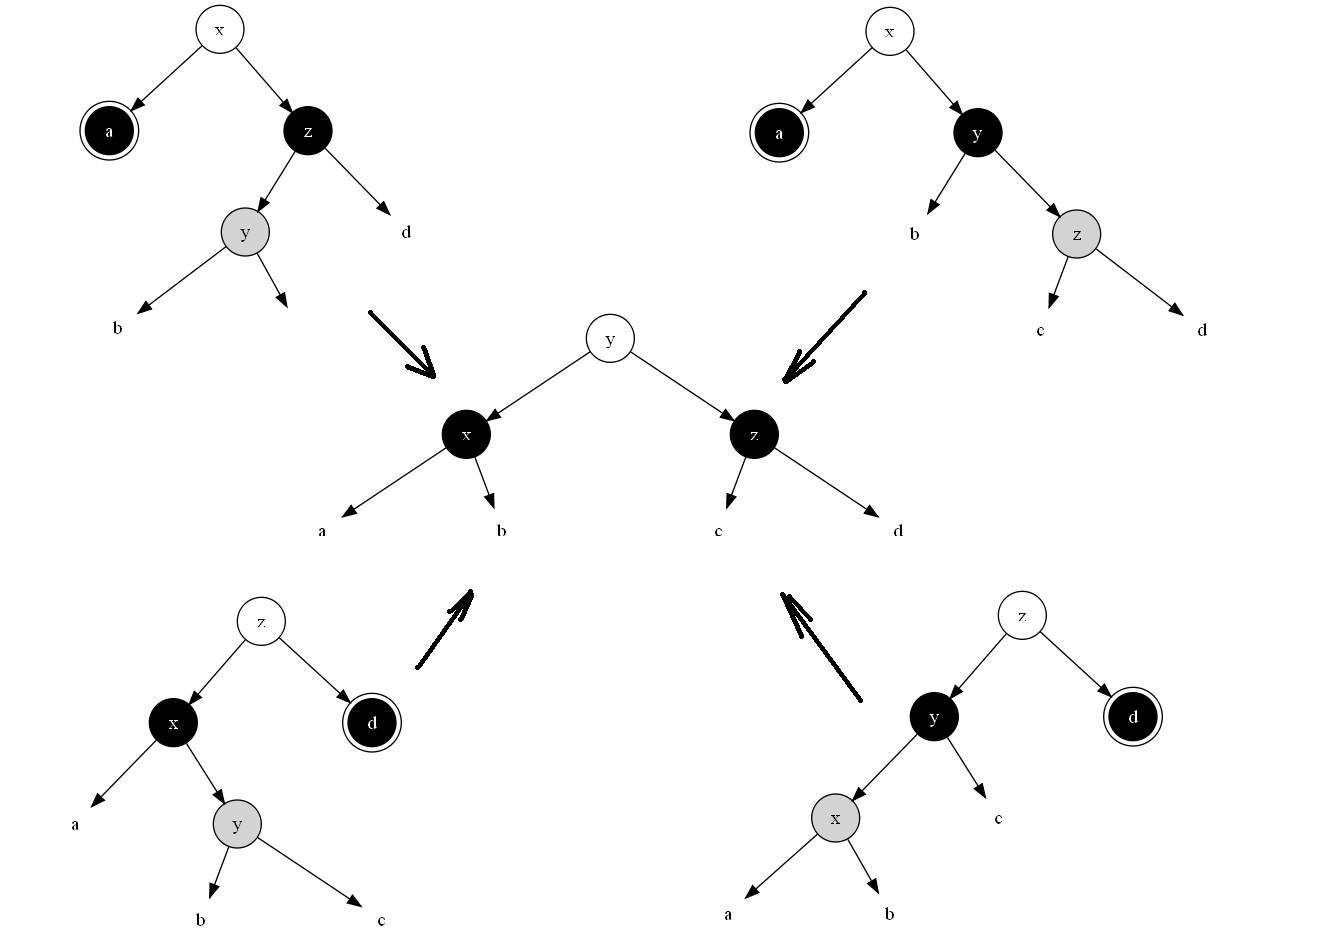
\includegraphics[scale=0.4]{img/del-case1.eps}
        \caption{case 1, fix the doubly black by rotation} \label{fig:del-case1}
       \end{center}
\end{figure}

In the figure, the doubly black node are shown in black circle with 2 edges.

After these 4 cases, the program entered another case. In this case, not only the sibling
of the doubly black node is black, but also its two children are black. We can change to color
of the sibling node to red and propagate the doubly black one level up to the parent node.

Let's review the 2 lines which are applied to this case. They are shown in figure \ref{fig:del-case2}.

\begin{lstlisting}
-- the sibling and its 2 children are all black, propagate the blackness up
fixDB color a@(Node BB _ _ _) x (Node B b@(Node B _ _ _) y c@(Node B _ _ _))
    = makeBlack (Node color (makeBlack a) x (Node R b y c))
fixDB color (Node B a@(Node B _ _ _) x b@(Node B _ _ _)) y c@(Node BB _ _ _)
    = makeBlack (Node color (Node R a x b) y (makeBlack c))
\end{lstlisting}

\begin{figure}[htbp]
       \begin{center}
	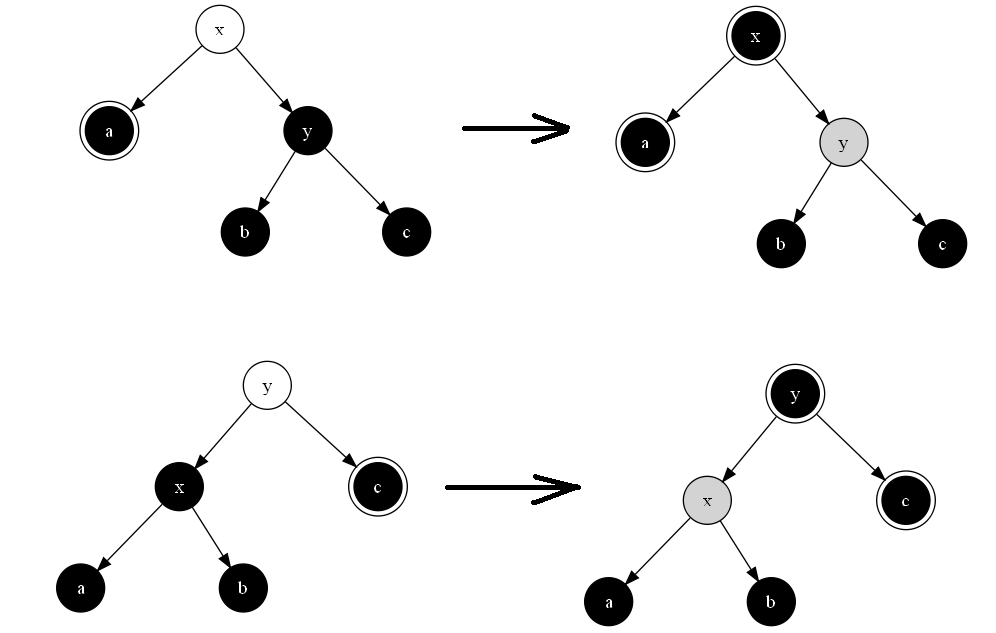
\includegraphics[scale=0.4]{img/del-case2.eps}
        \caption{case 2, propagate the blackness up.} \label{fig:del-case2}
       \end{center}
\end{figure}

These two cases are described in CLRS as case 2.

Next, we entered the final case. In this case, the sibling of the doubly black node is red.
We can do a rotation to change this case to case 1. the source code and the figures are shown
as below.

\begin{lstlisting}
-- the sibling is red
fixDB B a@(Node BB _ _ _) x (Node R b y c) = fixDB B (fixDB R a x b) y c
fixDB B (Node R a x b) y c@(Node BB _ _ _) = fixDB B a x (fixDB R b y c)
\end{lstlisting}

\begin{figure}[htbp]
       \begin{center}
	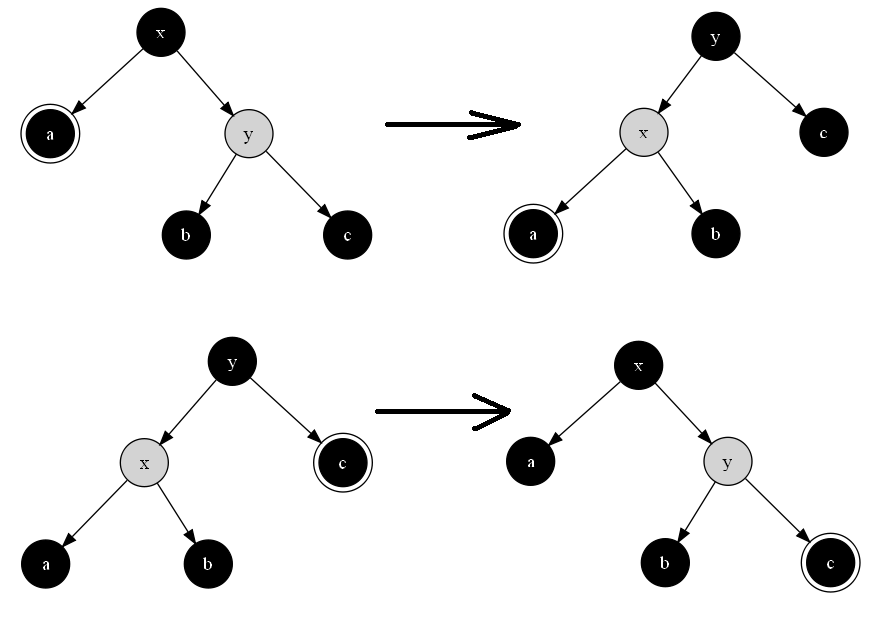
\includegraphics[scale=0.4]{img/del-case3.eps}
        \caption{case 3, the sibling of the doubly black is red.} \label{fig:del-case3}
       \end{center}
\end{figure}

This two cases are described in CLRS as case 1.

By fixing the doubly black node with the above 3 cases, There are two termination conditions
which the program will stop at. One is the case 1, The doubly black node was eliminated. The
other 2 cases may continuously propagate the doubly black node from bottom to top till the root.
Finally the program will mark the root node as black anyway, so the doubly blackness will be
removed.

we can test this delete program by using the following test cases:

\begin{lstlisting}
t1=listToRBTree [11, 2, 14, 1, 7, 15, 5, 8, 4]

testDel = "\ntest del 4: " ++ show (delete t1 4) ++
          "\ntest del 5: " ++ show (delete t1 5) ++
          "\ntest del 2: " ++ show (delete t1 2) ++
          "\ntest del 7: " ++ show (delete t1 7) ++
          "\ntest del 14: " ++ show (delete t1 14)

main = do
  putStrLn testDel
\end{lstlisting}

The program will output the result as below.

\begin{verbatim}
test del 4: (((. 1:B .) 2:B (. 5:B .)) 7:B (((. 8:R .) 11:B .) 14:B (. 15:B .)))
test del 5: (((. 1:B .) 2:B (. 4:B .)) 7:B (((. 8:R .) 11:B .) 14:B (. 15:B .)))
test del 2: (((. 1:B .) 4:B (. 5:B .)) 7:B (((. 8:R .) 11:B .) 14:B (. 15:B .)))
test del 7: (((. 1:B .) 2:B ((. 4:R .) 5:B .)) 8:B ((. 11:B .) 14:B (. 15:B .)))
test del 14: (((. 1:B .) 2:B ((. 4:R .) 5:B .)) 7:B (((. 8:R .) 11:B .) 15:B .))
\end{verbatim}

\subsubsection*{Python deletion, imperative}

Imperative deletion method is well discussed in CLRS. Since I added some helper member functions
in the red black tree definition. The delete method without the fixing part can be much simpler
than the one I give in \cite{bst-lxy}. Similar to the functional approach, I explicitly defined
the doubly black concept.

\lstset{language=Python}
\begin{lstlisting}
RED = 0
BLACK = 1
DOUBLY_BLACK = 2
\end{lstlisting}

There is small trick if I define doubly black color as integer 2, I can use color+1 to represent
doubly blackness later.

\lstset{language=Python}
\begin{lstlisting}
def rb_delete(t, x):
    if x is None: return t
    (parent, db) = (x.parent, None)
    if x.left is None:
        x.replace_by(x.right)
        db=x.right
    elif x.right is None:
        x.replace_by(x.left)
        db=x.left
    else:
        y = tree_min(x.right)
        (parent, db)=(y.parent, y.right)
        x.key = y.key
        y.replace_by(y.right)
        x=y
    if x.color == BLACK:
        t=rb_delete_fix(t, make_black(parent, db))
    remove_node(x)
    return t
\end{lstlisting}

The major difference is in the tail part. If the sliced out node is black, the program will
try a fixing procedure to re-balance the red black tree. The parameter pass to the fixing
function includes the tree and the doubly black node. In order to locate the doubly black
node. I provide a function make\_black(). It is implemented like this.

\begin{lstlisting}
def make_black(parent, x):
    if x is None:
        if is_leaf(parent):
            parent.color = DOUBLY_BLACK
        return parent
    else:
        x.color = x.color + 1
        return x

def is_leaf(x):
    if x is None: return False
    return (x.left is None) and (x.right is None)
\end{lstlisting}

In the delete function, I use parent to record the parent pointer of the node to be deleted. 
And variable db is point to the root of the sub tree which will replace x. db may be empty.
make\_black() function will check this predication. If it (the db) is empty, and the parent is a leaf
node (which means parent has a one child empty and another child doubly black empty), we make
the parent node doubly black. else we change the color of it (the db) to either black or doubly
black by increasing the color value by 1. please refer to the BBEmpty section in functional 
implementation for detail.

This delete function also use some read-only querying method, such as tree\_min(), they are defined
as same as in \cite{bst-lxy}. Let's review them again.

\begin{lstlisting}
def tree_min(t):
    while(t!=None and t.left != None):
        t = t.left
    return t

def remove_node(x):
    if (x is None): return
    x.parent = x.left = x.right = None

def tree_search(t, x):
    while(t!=None and t.key != x):
        if(x < t.key): t = t.left
        else: t = t.right
    return t
\end{lstlisting}

Next we go to the core function of the delete fixing procedure. Basically it is strictly implemented
based on CLRS.

\begin{lstlisting}
def rb_delete_fix(t, db):
    if db is None: return None # remove the root from a leaf tree
    while(db!=t and db.color==DOUBLY_BLACK):
        if db.sibling() != None:
            # case 1:  the sibling is red, (transform to make it black)
            if is_red(db.sibling()): 
                set_color([db.parent, db.sibling()],[RED, BLACK])
                if(db == db.parent.left):
                    t=left_rotate(t, db.parent)
                else:
                    t=right_rotate(t, db.parent)
            # case 3, 4: the sibling is black, and one nephew is red
            elif is_black(db.sibling()) and is_red(db.sibling().left): 
                if db == db.parent.left:
                    colors=[BLACK, BLACK, db.parent.color]
                    set_color([db, db.parent, 
                                   db.sibling().left], colors)
                    t=right_rotate(t, db.sibling())
                    t=left_rotate(t, db.parent)
                else:
                    colors=[BLACK, BLACK, db.parent.color, BLACK]
                    set_color([db, db.parent, db.sibling(), 
                                   db.sibling().left], colors)
                    t=right_rotate(t, db.parent)
            elif is_black(db.sibling()) and is_red(db.sibling().right):
                if db == db.parent.left:
                    colors=[BLACK, BLACK, db.parent.color, BLACK]
                    set_color([db, db.parent, db.sibling(), 
                                   db.sibling().right], colors)
                    t=left_rotate(t, db.parent)
                else:
                    colors=[BLACK, BLACK, db.parent.color]
                    set_color([db, db.parent, db.sibling().right], colors)
                    t=left_rotate(t, db.sibling())
                    t=right_rotate(t, db.parent)
            # case 2: the sibling and both nephews are black. 
            # (move the blackness up)
            elif is_black(db.sibling()) and (not is_red(db.sibling().left)) 
                   and (not is_red(db.sibling().right)):
               set_color([db, db.sibling()], [BLACK, RED])
               db.parent.color=db.parent.color+1
               db = db.parent
            # a sibling without child is invalid case, because it 
            # violate property 5
        else: # no sibling, we can move blackness up
            db.color = BLACK
            db.parent.color = db.parent.color+1
            db = db.parent
    t.color=BLACK
    return t
\end{lstlisting}

There is a slight difference from CLRS, I found either the sibling is on the left or on
the right, case 1 in the program can be applied in same way, so I pulled it up. There are
also 2 helper function to test if a node is red node or black node as below.

\begin{lstlisting}
def is_red(x):
    if x is None: return False
    return x.color == RED

def is_black(x):
    if x is None: return False
    return x.color == BLACK
\end{lstlisting}

In order to test the delete function for red black tree, I defined some similar helper
functions. The test cases are something like below.

\begin{lstlisting}
class Test:
    ...
    def __assert(self, msg, x, y):
        if(x == y): msg = msg + "OK."
        else: msg = msg + str(x) + "!=" + str(y) + "Fail."
        print msg

    def __test_del_n(self, tree, n):
        t = rbtree_clone(tree)
        t = rb_delete(t, tree_search(t, n))
        print "del ", n, ": ", rbtree_to_str(t)
        self.__assert("search after del: ", tree_search(t, n), None)

    def test_delete(self):
        for i in range(1, 10):
            self.__test_del_n(self.t1, i)
        self.__test_del_n(self.t1, 11) #del a non-exist value
        t = Node(1, BLACK) #leaf case
        self.__test_del_n(t, 1)
\end{lstlisting}

It will output the result in console.

\begin{verbatim}
del  1 :  ((. 2:R ((. 3:R .) 4:B .)) 5:B ((. 6:B .) 7:R ((. 8:R .) 9:B .)))
search after del: OK.
del  2 :  (((. 1:B .) 3:R (. 4:B .)) 5:B ((. 6:B .) 7:R ((. 8:R .) 9:B .)))
search after del: OK.
del  3 :  (((. 1:B .) 2:R (. 4:B .)) 5:B ((. 6:B .) 7:R ((. 8:R .) 9:B .)))
search after del: OK.
del  4 :  (((. 1:B .) 2:R (. 3:B .)) 5:B ((. 6:B .) 7:R ((. 8:R .) 9:B .)))
search after del: OK.
del  5 :  (((. 1:B .) 2:R ((. 3:R .) 4:B .)) 6:B (. 7:R ((. 8:R .) 9:B .)))
search after del: OK.
del  6 :  (((. 1:B .) 2:R ((. 3:R .) 4:B .)) 5:B (. 7:R ((. 8:R .) 9:B .)))
search after del: OK.
del  7 :  (((. 1:B .) 2:R ((. 3:R .) 4:B .)) 5:B ((. 6:B .) 8:R (. 9:B .)))
search after del: OK.
del  8 :  (((. 1:B .) 2:R ((. 3:R .) 4:B .)) 5:B ((. 6:B .) 7:R (. 9:B .)))
search after del: OK.
del  9 :  (((. 1:B .) 2:R ((. 3:R .) 4:B .)) 5:B ((. 6:B .) 7:R (. 8:B .)))
search after del: OK.
del  11 :  (((. 1:B .) 2:R ((. 3:R .) 4:B .)) 5:B ((. 6:B .) 7:R ((. 8:R .) 9:B .)))
search after del: OK.
del  1 :  .
search after del: OK.
\end{verbatim}

\subsubsection*{Scheme/Lisp deletion, functional}

Scheme/Lisp version of red-black tree deletion need more logical conditions 
without pattern matching. I defined some delete specific helper functions first.

\lstset{language=lisp}
\begin{lstlisting}
(define (dblack? t)
  (if (null? t) '() (equal? (color t) "BB")))

(define (set-color c t)
  (make-rbtree c (left t) (key t) (right t)))

(define (leaf? x)
  (if (null? x) '() (and (null? (left x)) (null? (right x)))))

(define (make-black parent t)
  (if (null? t)
      (if (leaf? parent) (set-color "BB" parent) parent)
      (if (red? t) (set-color "B" t) (set-color "BB" t))))

(define (tree-min tree) 
  (if (null? (left tree)) 
      tree 
      (tree-min (left tree)))) 
\end{lstlisting}

Function dblack is used to test if a node is doubly black. As same as Haskell
and Python version, I used explicit doubly black color in implementation. Function
set-color actually doesn't change the color of a node, (so no ! in the function
name) it create a new tree with specified color. Function leaf can help
to test if a node has both its children empty.

Function make-black is more
similar to the python version than the Haskell version. It takes 2 parameters,
one is the parent node, the other is the node we want to make it black.
This function can cover the doubly black empty case. In such case, it will
change the color of the parent node as doubly black if necessary.

The last helper function tree-min is as same as the one in binary search tree
\cite{bst-lxy}. It can help to find the minimum value in a tree.

With these helper functions, I defined the delete function as the following.

\begin{lstlisting}
(define (rb-delete tree x) ;; x is a value, not a node
  (define (blacken-root t)
    (if (null? t) '() (set-color "B" t)))
  (define (del t x)
    (cond ((null? t) '())
	  ((< x (key t)) (fix-dblack (color t) 
				     (del (left t) x)
				     (key t)
				     (right t)))
	  ((> x (key t)) (fix-dblack (color t)
				     (left t)
				     (key t)
				     (del (right t) x)))
	  ((null? (left t)) (if (black? t)
				(make-black t (right t))
				(right t)))
	  ((null? (right t)) (if (black? t)
				 (make-black t (left t))
				 (left t)))
	  (else (let ((newkey (key (tree-min (right t)))))
		  (fix-dblack (color t)
			      (left t)
			      newkey
			      (del (right t) newkey))))))
  (blacken-root (del tree x)))
\end{lstlisting}

Compare this implementation with the Haskell one, we can find they
are very same to each other. Most of the part is similar to the 
normal binary search tree deletion, however, it must fix the red
black tree property violation if we slice a black node out.

The core function to fixing this violation is defined like this.

\begin{lstlisting}
(define (fix-dblack c l k r)
  (cond 
   ;;case 1, the sibling is black, and it has one red child
   ((and (dblack? l) (black? r) (red? (left r)))
    (make-rbtree c 
		 (make-rbtree "B" (set-color "B" l) k (left (left r)))
		 (key (left r))
		 (make-rbtree "B" (right (left r)) (key r) (right r))))
   ((and (dblack? l) (black? r) (red? (right r)))
    (make-rbtree c
		 (make-rbtree "B" (set-color "B" l) k (left r))
		 (key r)
		 (set-color "B" (right r))))
   ((and (dblack? r) (black? l) (red? (right l)))
    (make-rbtree c
		 (make-rbtree "B" (left l) (key l) (left (right l)))
		 (key (right l))
		 (make-rbtree "B" (right (right l)) k (set-color "B" r))))
   ((and (dblack? r) (black? l) (red? (left l)))
    (make-rbtree c
		 (set-color "B" (left l))
		 (key l)
		 (make-rbtree "B" (right l) k (set-color "B" r))))
   ;;case 2, the sibling and its 2 children are all black,
   ;;        propagate the blackness up
   ((and (dblack? l) (black? r) (black? (left r)) (black? (right r)))
    (make-black '() (make-rbtree c
				 (set-color "B" l)
				 k
				 (set-color "R" r))))
   ((and (dblack? r) (black? l) (black? (left l)) (black? (right l)))
    (make-black '() (make-rbtree c
				 (set-color "R" l)
				 k
				 (set-color "B" r))))
   ;;case 3, the silbing is red
   ((and (dblack? l) (red? r))
    (fix-dblack "B" (fix-dblack "R" l k (left r)) (key r) (right r)))
   ((and (dblack? r) (red? l))
    (fix-dblack "B" (left l) (key l) (fix-dblack "R" (right l) k r)))
   (else (make-rbtree c l k r))))
\end{lstlisting}

Here is all about red black tree deletion in Scheme/Lisp. We can
test it with the following cases.

\begin{lstlisting}
(define (test-del) 
  (display (rb-delete t1 4)) (newline) 
  (display (rb-delete t1 5)) (newline) 
  (display (rb-delete t1 2)) (newline) 
  (display (rb-delete t1 7)) (newline) 
  (display (rb-delete t1 14)) (newline) 
  (display (rb-delete t1 3)))
\end{lstlisting}

If we evaluate the test-del in scheme R-E-P-L, the results are shown
like this.

\begin{verbatim}
(test-del)
(((() 1 B ()) 2 B (() 5 B ())) 7 B (((() 8 R ()) 11 B ()) 14 B (() 15 B ())))
(((() 1 B ()) 2 B (() 4 B ())) 7 B (((() 8 R ()) 11 B ()) 14 B (() 15 B ())))
(((() 1 B ()) 4 B (() 5 B ())) 7 B (((() 8 R ()) 11 B ()) 14 B (() 15 B ())))
(((() 1 B ()) 2 B ((() 4 R ()) 5 B ())) 8 B ((() 11 B ()) 14 B (() 15 B ())))
(((() 1 B ()) 2 B ((() 4 R ()) 5 B ())) 7 B ((() 8 B ()) 11 B (() 15 B (() 15 B ()))))
(((() 1 B ()) 2 B ((() 4 R ()) 5 B ())) 7 B (((() 8 R ()) 11 B ()) 14 B (() 15 B ())))
\end{verbatim}

The results are identify with the one output by Haskell.

\subsubsection*{C++ red black tree deletion}

I left C++ version of delete be the last one in this post because it
is most complex part. 
In C++ SGI STL, red black tree is deleted by passing a iterator as the
parameter. It represents the position where the node should be
deleted.

\lstset{language=C++}
\begin{lstlisting}
template <class _Key, class _Value, ...>
inline void _Rb_tree<_Key, ...>
  ::erase(iterator __position)
{
  _Link_type __y = 
    (_Link_type) _Rb_tree_rebalance_for_erase(__position._M_node,
                                              _M_header->_M_parent,
                                              _M_header->_M_left,
                                              _M_header->_M_right);
  destroy_node(__y);
  --_M_node_count;
}
\end{lstlisting}

The core algorithm is located in the rebalace for erase function as
the following.

\begin{lstlisting}
inline _Rb_tree_node_base*
_Rb_tree_rebalance_for_erase(_Rb_tree_node_base* __z,
                             _Rb_tree_node_base*& __root,
                             _Rb_tree_node_base*& __leftmost,
                             _Rb_tree_node_base*& __rightmost)
{
  _Rb_tree_node_base* __y = __z;
  _Rb_tree_node_base* __x = 0;
  _Rb_tree_node_base* __x_parent = 0;
  if (__y->_M_left == 0)     // __z has at most one non-null child. y == z.
    __x = __y->_M_right;     // __x might be null.
  else
    if (__y->_M_right == 0)  // __z has exactly one non-null child. y == z.
      __x = __y->_M_left;    // __x is not null.
    else {                   // __z has two non-null children.  Set __y to
      __y = __y->_M_right;   //   __z's successor.  __x might be null.
      while (__y->_M_left != 0)
        __y = __y->_M_left;
      __x = __y->_M_right;
    }
  if (__y != __z) {          // relink y in place of z.  y is z's successor
    __z->_M_left->_M_parent = __y; 
    __y->_M_left = __z->_M_left;
    if (__y != __z->_M_right) {
      __x_parent = __y->_M_parent;
      if (__x) __x->_M_parent = __y->_M_parent;
      __y->_M_parent->_M_left = __x;      // __y must be a child of _M_left
      __y->_M_right = __z->_M_right;
      __z->_M_right->_M_parent = __y;
    }
    else
      __x_parent = __y;  
    if (__root == __z)
      __root = __y;
    else if (__z->_M_parent->_M_left == __z)
      __z->_M_parent->_M_left = __y;
    else 
      __z->_M_parent->_M_right = __y;
    __y->_M_parent = __z->_M_parent;
    __STD::swap(__y->_M_color, __z->_M_color);
    __y = __z;
    // __y now points to node to be actually deleted
  }
  else {                        // __y == __z
    __x_parent = __y->_M_parent;
    if (__x) __x->_M_parent = __y->_M_parent;   
    if (__root == __z)
      __root = __x;
    else 
      if (__z->_M_parent->_M_left == __z)
        __z->_M_parent->_M_left = __x;
      else
        __z->_M_parent->_M_right = __x;
    if (__leftmost == __z) 
      if (__z->_M_right == 0)        // __z->_M_left must be null also
        __leftmost = __z->_M_parent;
    // makes __leftmost == _M_header if __z == __root
      else
        __leftmost = _Rb_tree_node_base::_S_minimum(__x);
    if (__rightmost == __z)  
      if (__z->_M_left == 0)         // __z->_M_right must be null also
        __rightmost = __z->_M_parent;  
    // makes __rightmost == _M_header if __z == __root
      else                      // __x == __z->_M_left
        __rightmost = _Rb_tree_node_base::_S_maximum(__x);
  }
  if (__y->_M_color != _S_rb_tree_red) { 
    while (__x != __root && (__x == 0 || __x->_M_color == _S_rb_tree_black))
      if (__x == __x_parent->_M_left) {
        _Rb_tree_node_base* __w = __x_parent->_M_right;
        if (__w->_M_color == _S_rb_tree_red) {
          __w->_M_color = _S_rb_tree_black;
          __x_parent->_M_color = _S_rb_tree_red;
          _Rb_tree_rotate_left(__x_parent, __root);
          __w = __x_parent->_M_right;
        }
        if ((__w->_M_left == 0 || 
             __w->_M_left->_M_color == _S_rb_tree_black) &&
            (__w->_M_right == 0 || 
             __w->_M_right->_M_color == _S_rb_tree_black)) {
          __w->_M_color = _S_rb_tree_red;
          __x = __x_parent;
          __x_parent = __x_parent->_M_parent;
        } else {
          if (__w->_M_right == 0 || 
              __w->_M_right->_M_color == _S_rb_tree_black) {
            if (__w->_M_left) __w->_M_left->_M_color = _S_rb_tree_black;
            __w->_M_color = _S_rb_tree_red;
            _Rb_tree_rotate_right(__w, __root);
            __w = __x_parent->_M_right;
          }
          __w->_M_color = __x_parent->_M_color;
          __x_parent->_M_color = _S_rb_tree_black;
          if (__w->_M_right) __w->_M_right->_M_color = _S_rb_tree_black;
          _Rb_tree_rotate_left(__x_parent, __root);
          break;
        }
      } else {                  // same as above, with _M_right <-> _M_left.
        _Rb_tree_node_base* __w = __x_parent->_M_left;
        if (__w->_M_color == _S_rb_tree_red) {
          __w->_M_color = _S_rb_tree_black;
          __x_parent->_M_color = _S_rb_tree_red;
          _Rb_tree_rotate_right(__x_parent, __root);
          __w = __x_parent->_M_left;
        }
        if ((__w->_M_right == 0 || 
             __w->_M_right->_M_color == _S_rb_tree_black) &&
            (__w->_M_left == 0 || 
             __w->_M_left->_M_color == _S_rb_tree_black)) {
          __w->_M_color = _S_rb_tree_red;
          __x = __x_parent;
          __x_parent = __x_parent->_M_parent;
        } else {
          if (__w->_M_left == 0 || 
              __w->_M_left->_M_color == _S_rb_tree_black) {
            if (__w->_M_right) __w->_M_right->_M_color = _S_rb_tree_black;
            __w->_M_color = _S_rb_tree_red;
            _Rb_tree_rotate_left(__w, __root);
            __w = __x_parent->_M_left;
          }
          __w->_M_color = __x_parent->_M_color;
          __x_parent->_M_color = _S_rb_tree_black;
          if (__w->_M_left) __w->_M_left->_M_color = _S_rb_tree_black;
          _Rb_tree_rotate_right(__x_parent, __root);
          break;
        }
      }
    if (__x) __x->_M_color = _S_rb_tree_black;
  }
  return __y;
}
\end{lstlisting}

In order to focus on the core algorithm, Let's put our eye on the
while loop. In case the deleted node is not red, it will break the red
black tree property number 5. Then we entered the while loop until
either we move the doubly blackness up to root or solved it only by
making color changes. Inside the while, be outer if-else each deal
with 3 cases. They are left-right symmetric to each other. Those 3
cases covers the sibling is red; the sibling and one nephew are black;
and the sibling with both nephew are all black.

\section{Appendix} \label{appendix}
%\appendix
All programs except the SGI STL C++ are provided along with this article. They are free for downloading.
\begin{itemize}
\item RBTree.hs, Haskell version of red black tree, with test cases. I compiled
and tested it with GHC 6.10.4.
\item rbtree.py, Python version of the red black tree, with test cases. Tested
with Python 2.5.1
\item rbtree.scm, Scheme version of the red black tree and test cases. Tested
with MIT/Scheme 14.9
\end{itemize}

SGI STL C++ implementation of red black tree can be found from here:
http://www.sgi.com/tech/stl/stl\_tree.h

Besides them, I use graphviz to draw most of the figures in this post. In order to
translate the red black tree output to dot language scripts. I wrote a python program.
it can be used like this.

\begin{verbatim}
./rbt2dot.py -o foo.dot "(((. 1:B .) 2:B .) 3:R ((. 4:B .) 5:B (. 6:B  .)))"
\end{verbatim}

This helper scripts can also be downloaded with this article.

download position: http://sites.google.com/site/algoxy/rbtree/rbtree.zip

\begin{thebibliography}{99}

\bibitem{CLRS}
Thomas H. Cormen, Charles E. Leiserson, Ronald L. Rivest and Clifford Stein. 
``Introduction to Algorithms, Second Edition''. ISBN:0262032937. The MIT Press. 2001

\bibitem{okasaki}
Chris Okasaki. ``FUNCTIONAL PEARLS Red-Black Trees in a Functional Setting''. J. Functional Programming. 1998

\bibitem{bst-lxy}
Liu Xinyu. ``Comparison of imperative and functional implementation of binary search tree''. http://sites.google.com/site/algoxy/bstree

\bibitem{wiki}
Wikipedia. ``Red-black tree''. http://en.wikipedia.org/wiki/Red-black\_tree

\bibitem{lyn}
Lyn Turbak. ``Red-Black Trees''. cs.wellesley.edu/~cs231/fall01/red-black.pdf Nov. 2, 2001.

\bibitem{sgi-stl}
http://www.sgi.com/tech/stl/

\bibitem{hj-stl}
Hou Jie. ``The annotated STL sources (using SGI STL)''. ISBN:7-5609-2699-1 http://press.hust.edu.cn. 2002.

\end{thebibliography}

\ifx\wholebook\relax\else
\end{document}
\fi
